\documentclass[t]{beamer}
%\documentclass[finnish,english,handout]{beamer}

% Uncomment if want to show notes
% \setbeameroption{show notes}

\mode<presentation>
{
  \usetheme{Copenhagen}
  % oder ...

  %\setbeamercovered{transparent}
  % oder auch nicht
}


\usepackage[T1]{fontenc}
\usepackage[latin1]{inputenc}
\usepackage{times}
\usepackage{epic,epsfig}
\usepackage{subfigure,float}
\usepackage{amsmath,amsfonts,amssymb}
\usepackage{inputenc}
\usepackage{afterpage}
\usepackage{url}
\urlstyle{same}
\usepackage{amsbsy}
\usepackage{eucal}
\usepackage{rotating}
\usepackage{listings}
\usepackage{lstbayes}
\usepackage[all,poly,ps,color]{xy}
\usepackage{eurosym}

\usepackage{natbib}
\bibliographystyle{apalike}

\hypersetup{%
  bookmarksopen=true,
  bookmarksnumbered=true,
  pdftitle={Stan},
  pdfsubject={Bayesian data analysis},
  pdfauthor={Aki Vehtari},
  pdfkeywords={},
  pdfstartview={FitH -32768},
  colorlinks=true,
  linkcolor=navyblue,
  citecolor=navyblue,
  filecolor=navyblue,
  urlcolor=navyblue
}

% \definecolor{hutblue}{rgb}{0,0.2549,0.6784}
% \definecolor{midnightblue}{rgb}{0.0977,0.0977,0.4375}
% \definecolor{hutsilver}{rgb}{0.4863,0.4784,0.4784}
% \definecolor{lightgray}{rgb}{0.95,0.95,0.95}
% \definecolor{section}{rgb}{0,0.2549,0.6784}
% \definecolor{list1}{rgb}{0,0.2549,0.6784}
\definecolor{forestgreen}{rgb}{0.1333,0.5451,0.1333}
\definecolor{navyblue}{rgb}{0,0,0.5}
\renewcommand{\emph}[1]{\textcolor{navyblue}{#1}}

\graphicspath{{./figs/}}

\pdfinfo{
  /Title      (Bayesian data analysis 9)
  /Author     (Aki Vehtari) %
  /Keywords   (Bayesian probability theory, Bayesian inference, Bayesian data analysis)
}


\parindent=0pt
\parskip=8pt
\tolerance=9000
\abovedisplayshortskip=0pt

\setbeamertemplate{navigation symbols}{}
\setbeamertemplate{headline}[default]{}
\setbeamertemplate{headline}[text line]{\insertsection}
\setbeamertemplate{footline}[frame number]


\def\o{{\mathbf o}}
\def\t{{\mathbf \theta}}
\def\w{{\mathbf w}}
\def\x{{\mathbf x}}
\def\y{{\mathbf y}}
\def\z{{\mathbf z}}

\def\peff{p_{\mathrm{eff}}}
\def\eff{\mathrm{eff}}

\DeclareMathOperator{\E}{E}
\DeclareMathOperator{\Var}{Var}
\DeclareMathOperator{\var}{var}
\DeclareMathOperator{\Sd}{Sd}
\DeclareMathOperator{\sd}{sd}
\DeclareMathOperator{\Gammad}{Gamma}
\DeclareMathOperator{\Invgamma}{Inv-gamma}
\DeclareMathOperator{\Bin}{Bin}
\DeclareMathOperator{\Negbin}{Neg-bin}
\DeclareMathOperator{\Poisson}{Poisson}
\DeclareMathOperator{\Beta}{Beta}
\DeclareMathOperator{\logit}{logit}
\DeclareMathOperator{\N}{N}
\DeclareMathOperator{\U}{U}
\DeclareMathOperator{\BF}{BF}
\DeclareMathOperator{\Invchi2}{Inv-\chi^2}
\DeclareMathOperator{\NInvchi2}{N-Inv-\chi^2}
\DeclareMathOperator{\InvWishart}{Inv-Wishart}
\DeclareMathOperator{\tr}{tr}
% \DeclareMathOperator{\Pr}{Pr}
\def\euro{{\footnotesize \EUR\, }}
\DeclareMathOperator{\rep}{\mathrm{rep}}

% \def\dashxy(#1){%
%   /xydash{[#1] 0 setdash}def}
% \def\grayxy(#1){%
%   /xycolor{#1 setgray}def}
% \newgraphescape{D}[1]{!{\ar @*{[!\dashxy(2 2)]} "#1"}}
% \newgraphescape{P}[1]{!{\ar "#1"}}
% \newgraphescape{F}[1]{!{*+=<2em>[F=]{#1}="#1"}}
% \newgraphescape{O}[1]{!{*+=<2em>[F]{#1}="#1"}}
% \newgraphescape{V}[1]{!{*+=<2em>[o][F]{#1}="#1"}}
% \newgraphescape{B}[3]{!{{ "#1"*+#3\frm{} }.{ "#2"*+#3\frm{} } *+[F:!\grayxy(0.75)]\frm{}}}


\title[]{Bayesian data analysis}
\subtitle{}

\author{Aki Vehtari}

\institute[Aalto]{}

\begin{document}

\begin{frame}

  {\Large\color{navyblue} Chapter 9}

  \begin{itemize}
\item 9.1 Context and basic steps (most important part)
\item 9.2 Example
\item 9.3 Multistage decision analysis (example)
\item 9.4 Hierarchical decision analysis (example)
\item 9.5 Personal vs. institutional decision analysis
\end{itemize}
\end{frame}

\begin{frame}

  {\Large\color{navyblue} Bayesian decision theory}

  \begin{itemize}
  \item<+-> Potential decisions $d$
    \begin{itemize}
      \item or actions $a$
    \end{itemize}
  \item<+-> Potential consequences $x$
    \begin{itemize}
      \item $x$ may be categorical, ordinal, real, scalar, vector, etc.
    \end{itemize}
  \item<+-> Probability distributions of consequences given decisions $p(x|d)$
    \begin{itemize}
    \item in decision making the decisions are controlled and thus $p(d)$ does not exist
    \end{itemize}
  \item<+->  Utility function $U(x)$ maps consequences to real value
    \begin{itemize}
      \item e.g. euro or expected lifetime
      \item instead of utility sometimes cost or loss is defined
    \end{itemize}
    \vspace{-1mm}
  \item<+-> Expected utility  $E[U(x)|d]=\int U(x) p(x|d) dx$
  \item<+-> Choose decision $d^*$, which maximizes the expected utility
    \begin{equation*}
      d^*=\arg\max_d E[U(x)|d]
    \end{equation*}
  \end{itemize}

\end{frame}

\begin{frame}

{\Large\color{navyblue} Example of decision making: 2 choices}

\begin{itemize}
\item<+-> Helen is going to pick mushrooms in a forest, while she notices a
  paw print which could made by a dog or a wolf
\item<+-> Helen measures that the length of the paw print is 14 cm and
  goes home to Google how big paws dogs and wolves have, and tries
  then to infer which animal has made the paw print
  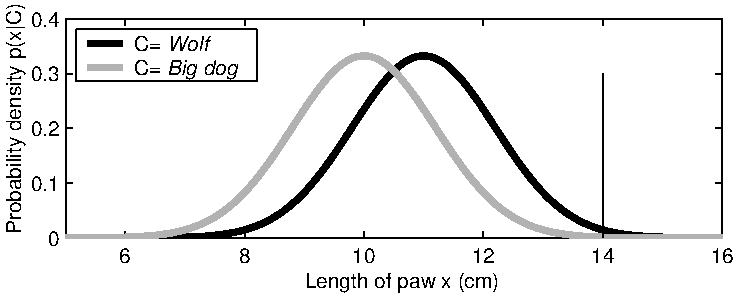
\includegraphics[width=11cm]{hatutus_likelihoods}
  observed length has been marked with a horizontal line
\item<+-> Likelihood of wolf is 0.92 (alternative being dog)
\end{itemize}

\end{frame}

\begin{frame}
  
{\Large\color{navyblue} Example of decision making}

  \begin{itemize}
  \item<+-> Helen assumes also that in her living area there are about one
    hundred times more free running dogs than wolves, that is {\em a
      priori} probability for wolf, before observation is 1\%.
  \item<+-> Likelihood and posterior
    \begin{center}\leavevmode
      \begin{tabular}{| l | c c |}
        \hline
        Animal &  Likelihood & Posterior probability \\
        \hline
        Wolf     &  0.92            & 0.10      \\
        Dog    &  0.08        & 0.90    \\
        \hline
      \end{tabular}
    \end{center}
  \item<+-> Posterior probability of wolf is 10\%
  \end{itemize}

\end{frame}

\begin{frame}

{\Large\color{navyblue} Example of decision making}

  \begin{itemize}
  \item<+-> Helen has to make decision whether to go pick mushrooms
  \item<+-> If she doesn't go to pick mushrooms utility is zero
  \item<+-> Helen assigns positive utility 1 for getting fresh mushrooms
  \item<+-> Helen assigns negative utility -1000 for a event that she goes to the forest and wolf attacks (for some reason Helen assumes that wolf will always attack)\\
    \vspace{\baselineskip}
    \uncover<+->{
    \begin{minipage}[t]{58mm}
      \small
      \begin{tabular}{| l | c c |}
        \hline
        & \multicolumn{2}{ c |}{Animal} \\
        Decision $d$           & Wolf & Dog \\
        \hline
        Stay home             & 0    & 0              \\
        Go to the forest      & -1000 & 1      \\
        \hline
      \end{tabular}\\
      {Utility matrix $U(x)$}
    \end{minipage}
    }
    ~\\
    \vspace{\baselineskip}
    \uncover<+->{
    \begin{minipage}[t]{58mm}
      \small
      \begin{tabular}{| l | c | }
        \hline
        & Conditional utility \\
        Action $d$        &  $E[U(x)|d]$ \\
        \hline
        Stay home         &  0       \\
        Go to the forest  &  -100+0.9     \\
        \hline
      \end{tabular}\\
      {Utilities for different actions}
    \end{minipage}
}
  \end{itemize}

\end{frame}

\begin{frame}
  
  {\Large\color{navyblue} Example of decision making}

  \begin{itemize}
  \item<+-> Maximum likelihood decision would be to assume that there is a wolf
  \item<+-> Maximum posterior decision would be to assume that there is a dog
  \item<+-> Maximum utility decision is to stay home, even if it is more likely that the animal is dog
  \item<+-> Example illustrates that the uncertainties (probabilities)
    related to all consequences need to be carried on until final
    decision making
  \end{itemize}

\end{frame}


\begin{frame}

{\Large\color{navyblue} Example of decision making: several choices}

\begin{itemize}
  \item Prof. Gelman has a jar of quarters
    \begin{itemize}
    \item he first drawed a line on the side of the jar and then
      filled the jar up to the line, and so the number coins was not
      chosen beforehand
    \item Prof. Gelman does not know the number of coins in the jar
    \item<2-> Prof. Gelman gives the class a chance to win the coins if
      they guess the number of coins correctly (someone else has
      counted the coins without telling Gelman)
    \item<2-> How should the students make the decision?
    \end{itemize}
\end{itemize}

\end{frame}

\begin{frame}

  {\Large\color{navyblue} Multi-stage decision making (Section 9.3)}

  \begin{itemize}
  \item<+-> 95 year old has a tumor that is malignant with 90\% probability
  \item<+-> Based on statistics
    \begin{itemize}
    \item<.-> expected lifetime is 34.8 months if no cancer
    \item<+-> expected lifetime is 16.7 months if cancer and radiation therapy is used
    \item<+-> expected liftime is 20.3 months if cancer and surgery, but the probability of dying in surgery is 35\% (for 95 year old)
    \item<+-> expected lifetime is 5.6 months is cabcer and no treatment
    \end{itemize}
  \item<+-> Which treatment to choose?
    \begin{itemize}
    \item<.-> quality adjusted life time
    \item<.-> 1 month is subtracted for the time spent in treatments
    \end{itemize}
   \item<+-> Quality adjusted life time
    \begin{itemize}
    \item<.-> Radiothreapy: 0.9*16.7 + 0.1*34.8 - 1 = 17.5mo
    \item<+-> Surgery: 0.35*0 + 0.65*(0.9*20.3 + 0.1*34.8 - 1) = 13.5mo
    \item<+-> No treatment: 0.9*5.6 + 0.1*34.8 = 8.5mo
    \end{itemize}
  \item<+-> See the book for continuation of the example with
    additional test for cancer
\end{itemize}

\end{frame}

\begin{frame}
  
  {\Large\color{navyblue} Design of experiment}

  \begin{itemize}
  \item Which experiment would give most additional information
    \begin{itemize}
    \item decide values $x_{n+1}$ for the next experiment
    \item which values of $x_{n+1}$ would reduce the posterior
      uncertainty most
    \end{itemize}
  \item Example
    \begin{itemize}
    \item Imagine that in bioassay the posterior uncertainty of LD50 is too large
    \item which dose should be used in the next experiment to reduce
      the variance of LD50 as much as possible ?
      \begin{itemize}
        \item this way less experiments need to be made (and less animals need to be killed)
      \end{itemize}
    \end{itemize}
  \end{itemize}
\end{frame}

\begin{frame}
  
  {\Large\color{navyblue} Bayesian optimization}

  \begin{itemize}
  \item Design of experiment
  \end{itemize}

\end{frame}

\begin{frame}
  
  {\Large\color{navyblue} Bayesian optimization}

    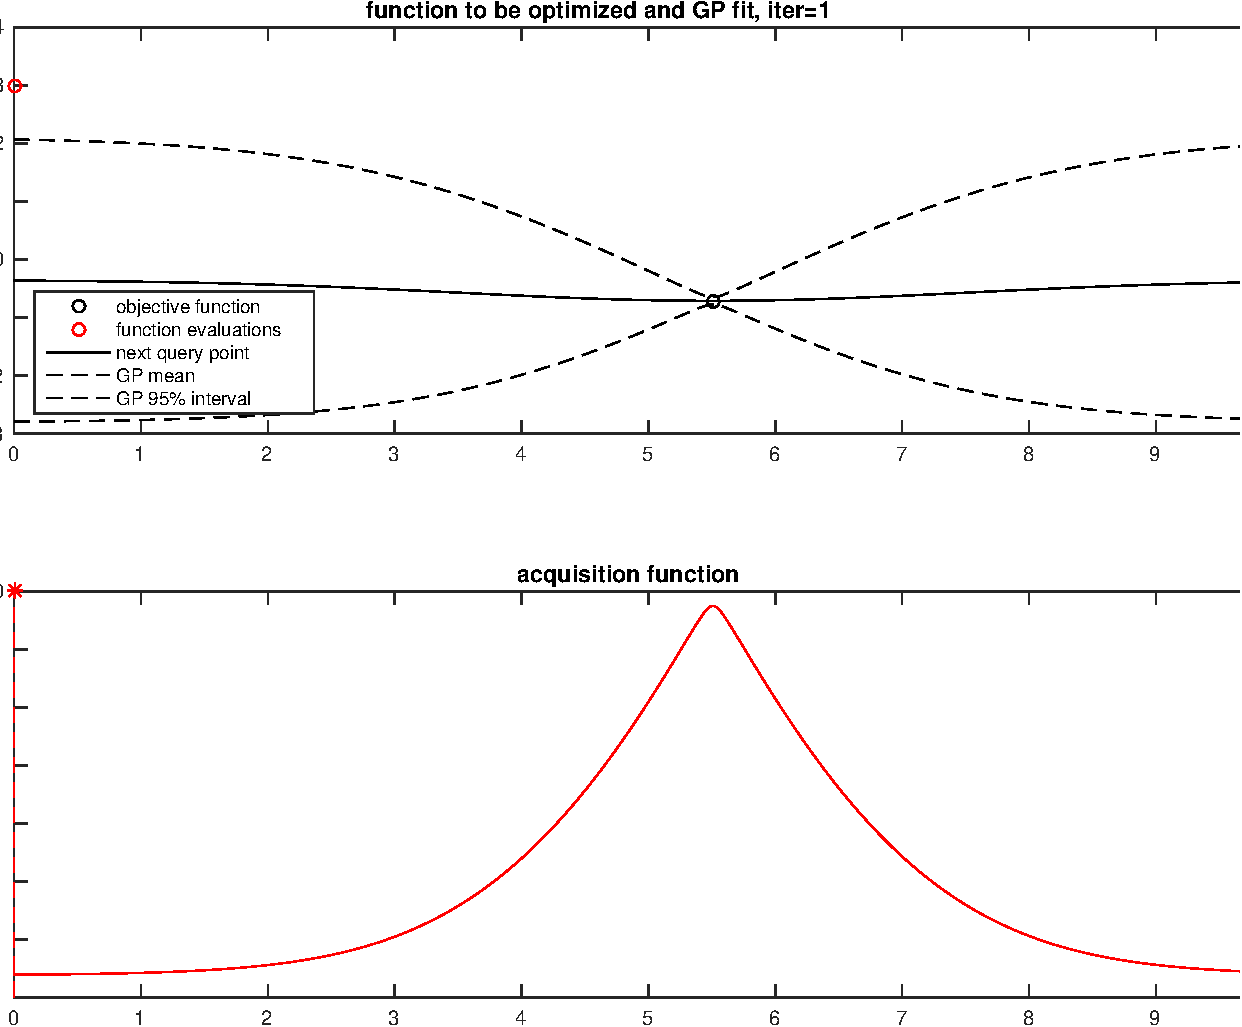
\includegraphics[width=10cm]{bayesopt_1d_regular_iter1-crop.pdf}

\end{frame}

\begin{frame}
  
  {\Large\color{navyblue} Bayesian optimization}

    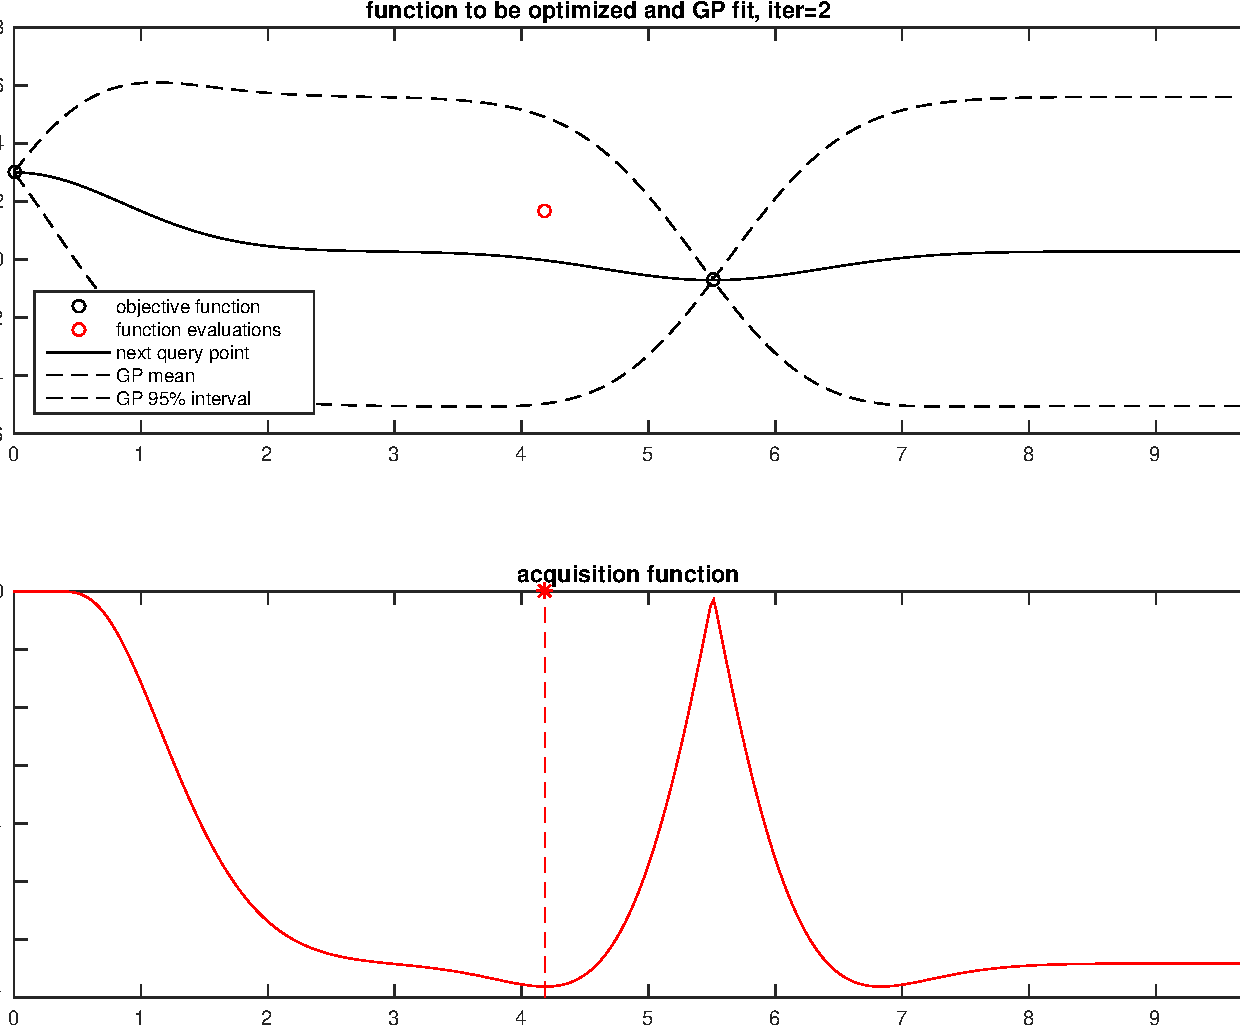
\includegraphics[width=10cm]{bayesopt_1d_regular_iter2-crop.pdf}

\end{frame}

\begin{frame}
  
  {\Large\color{navyblue} Bayesian optimization}

    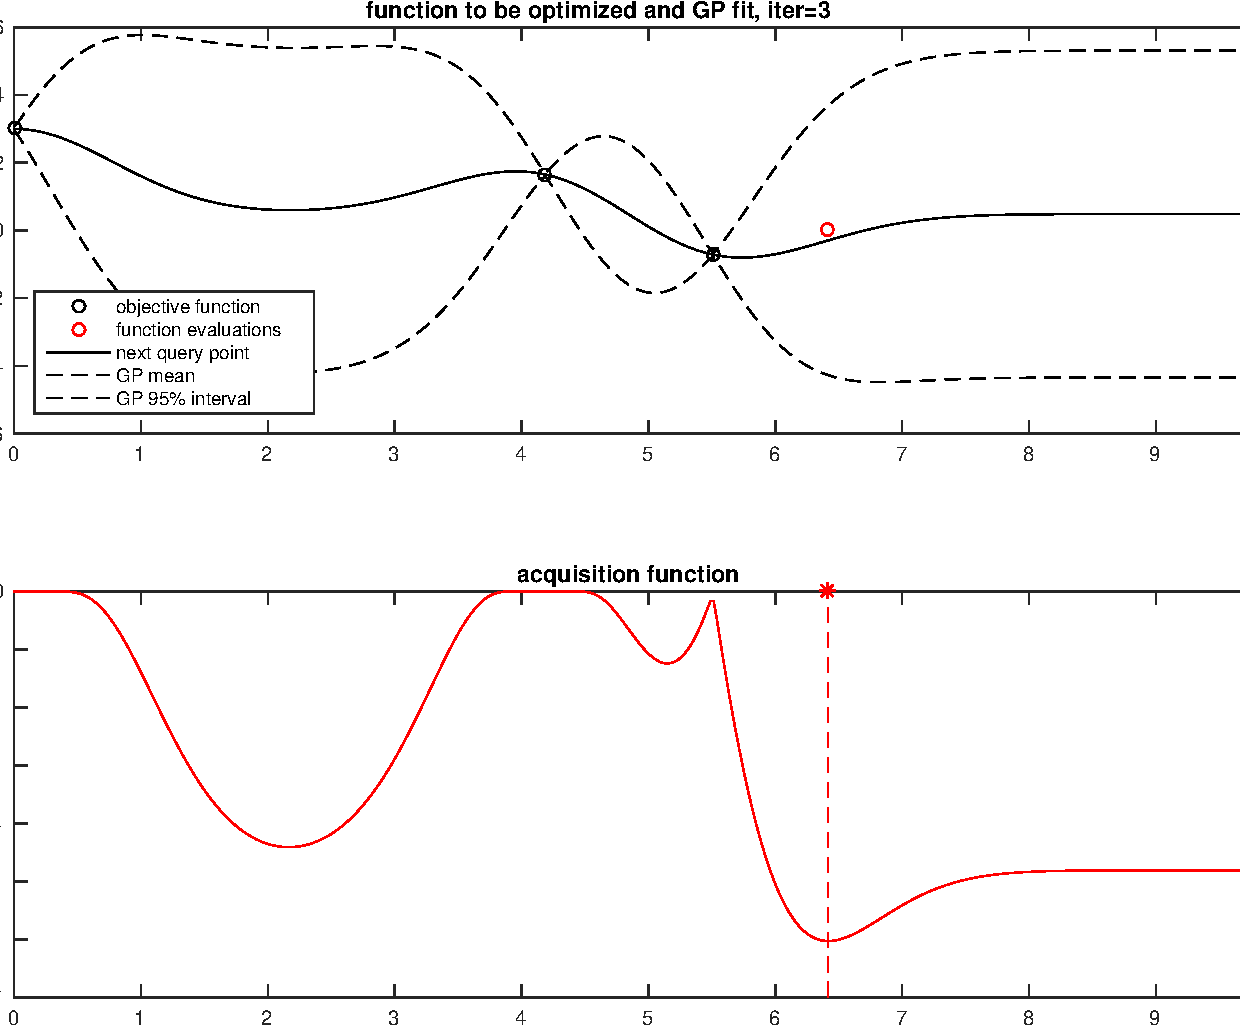
\includegraphics[width=10cm]{bayesopt_1d_regular_iter3-crop.pdf}

\end{frame}

\begin{frame}
  
  {\Large\color{navyblue} Bayesian optimization}

    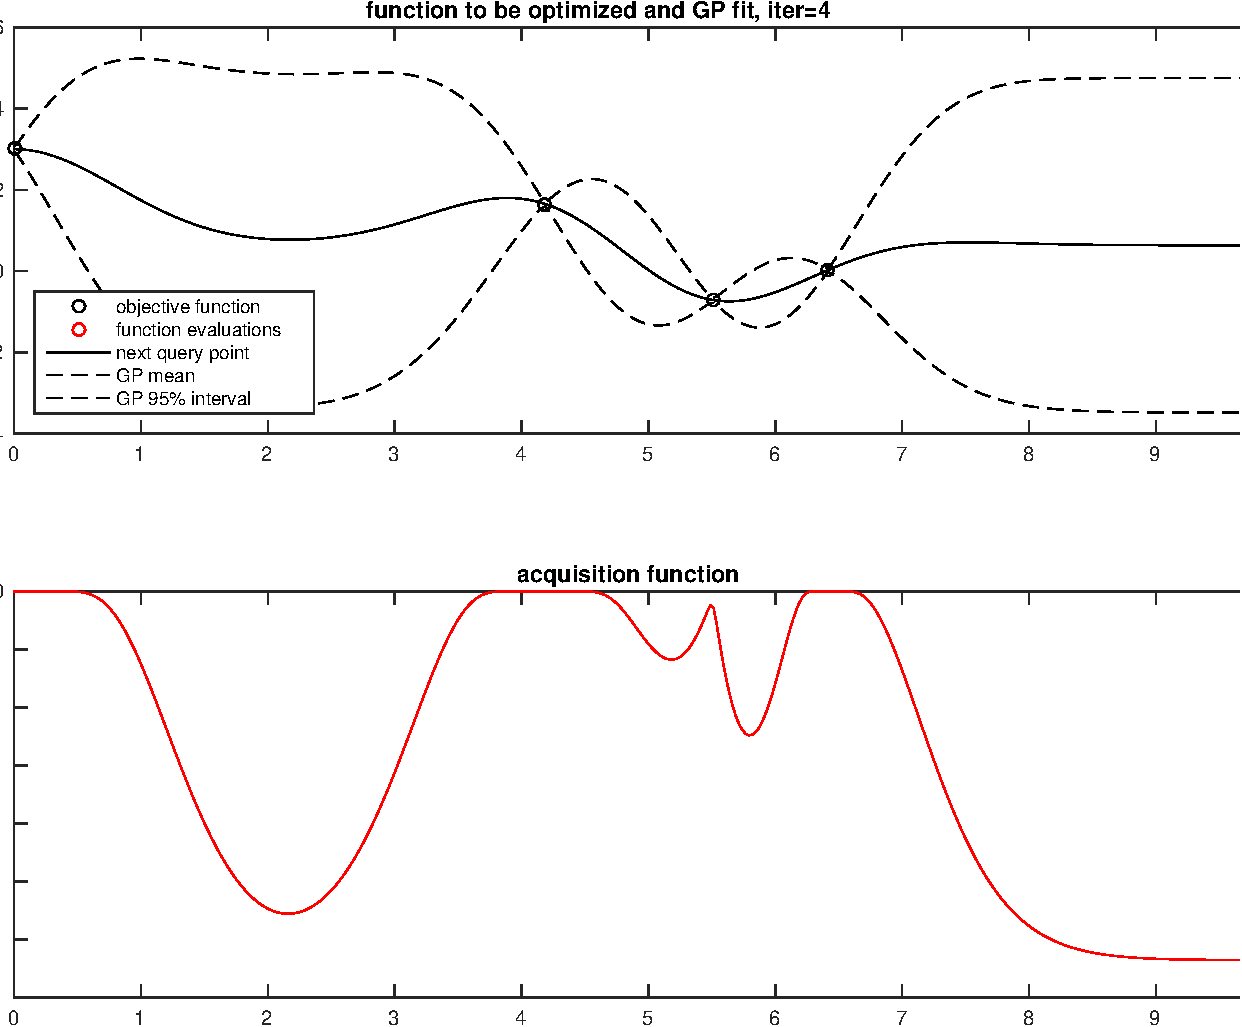
\includegraphics[width=10cm]{bayesopt_1d_regular_iter4-crop.pdf}

\end{frame}
\begin{frame}
  
  {\Large\color{navyblue} Bayesian optimization}

    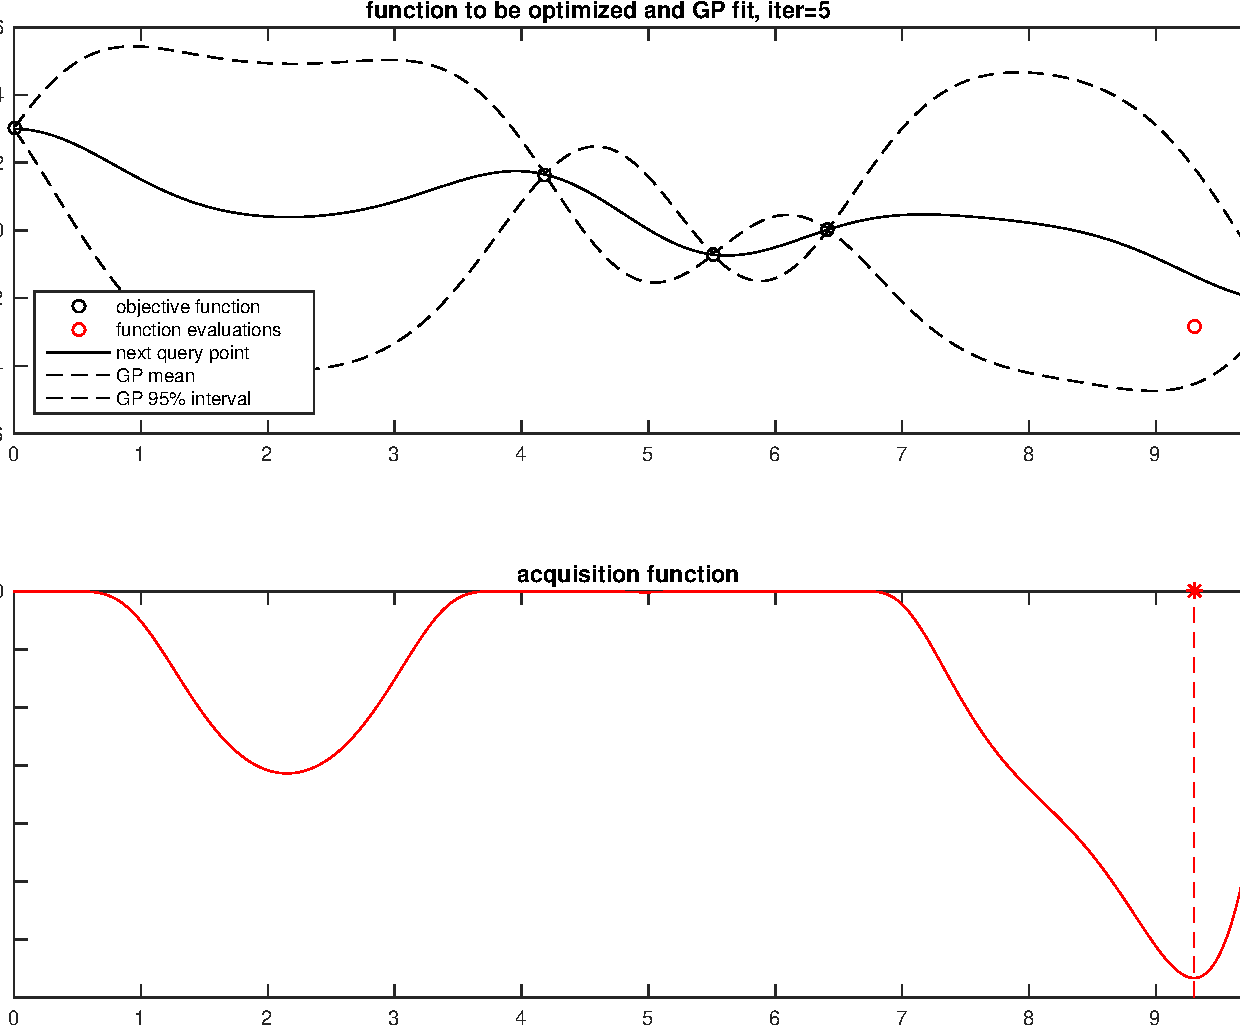
\includegraphics[width=10cm]{bayesopt_1d_regular_iter5-crop.pdf}

\end{frame}
\begin{frame}
  
  {\Large\color{navyblue} Bayesian optimization}

    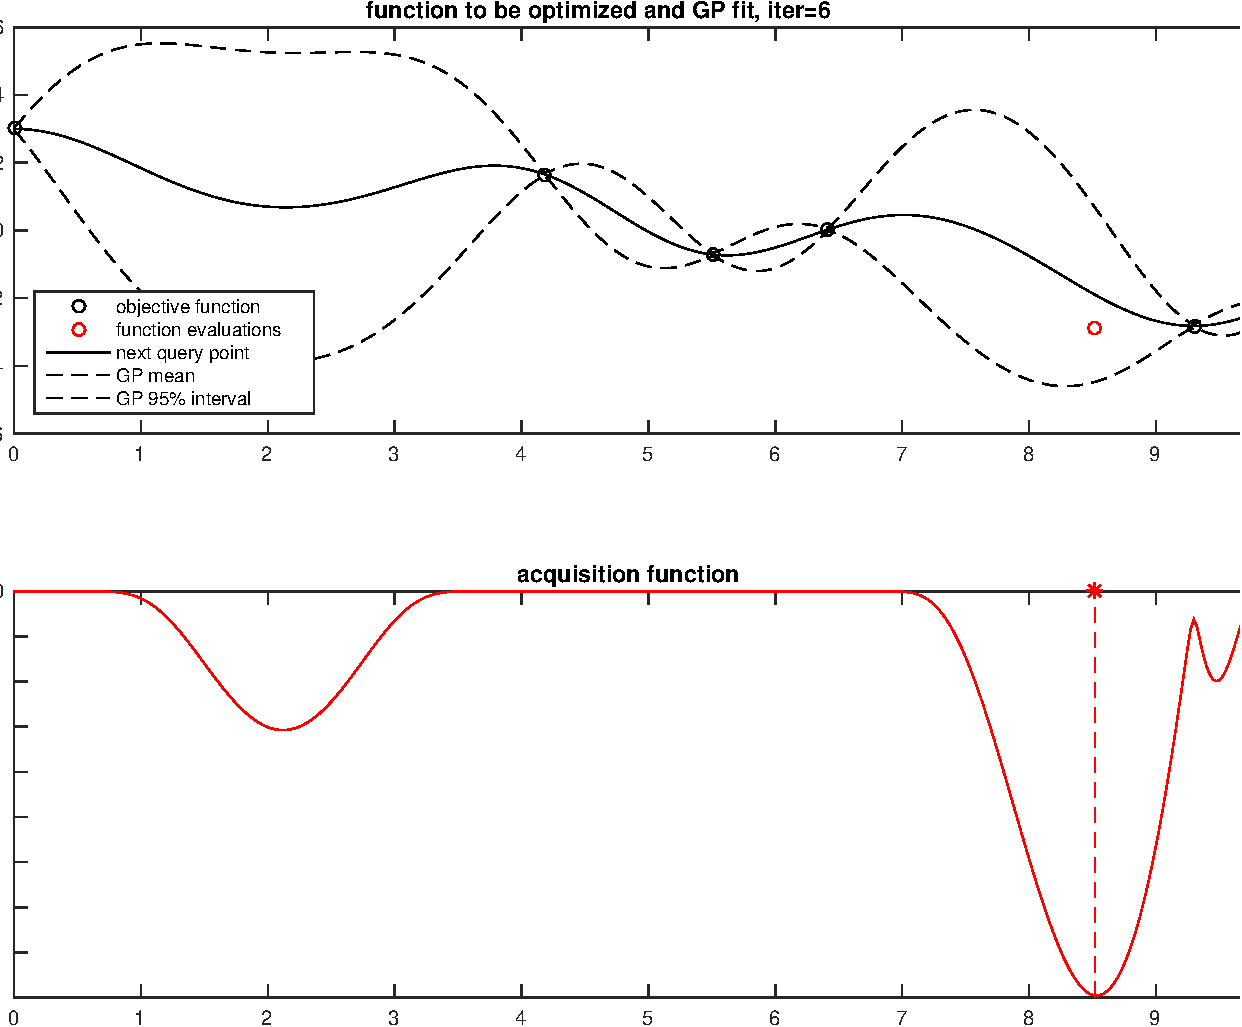
\includegraphics[width=10cm]{bayesopt_1d_regular_iter6-crop.pdf}

\end{frame}
\begin{frame}
  
  {\Large\color{navyblue} Bayesian optimization}

    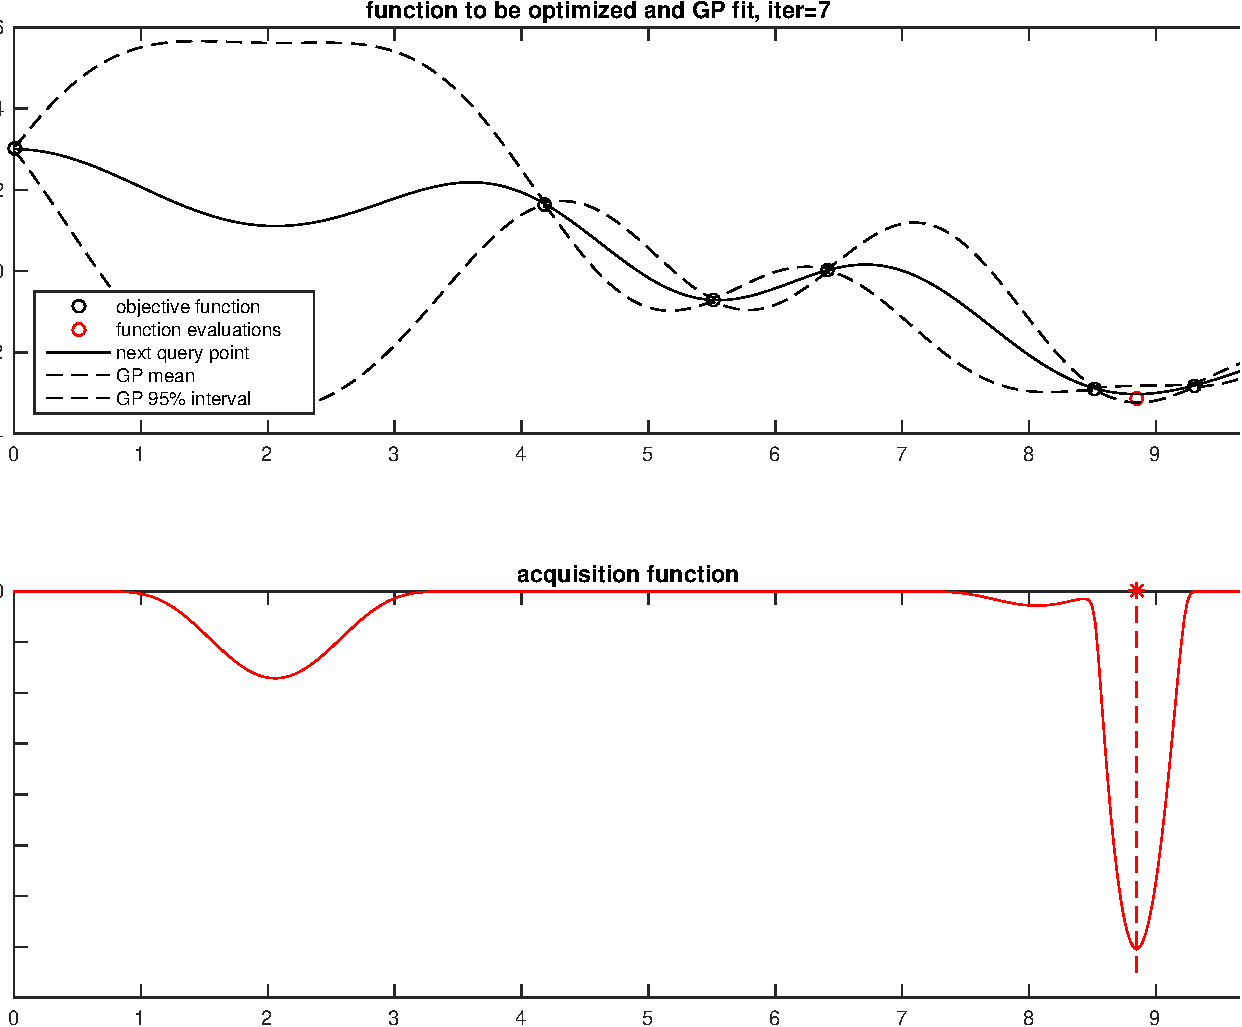
\includegraphics[width=10cm]{bayesopt_1d_regular_iter7-crop.pdf}

\end{frame}
\begin{frame}
  
  {\Large\color{navyblue} Bayesian optimization}

    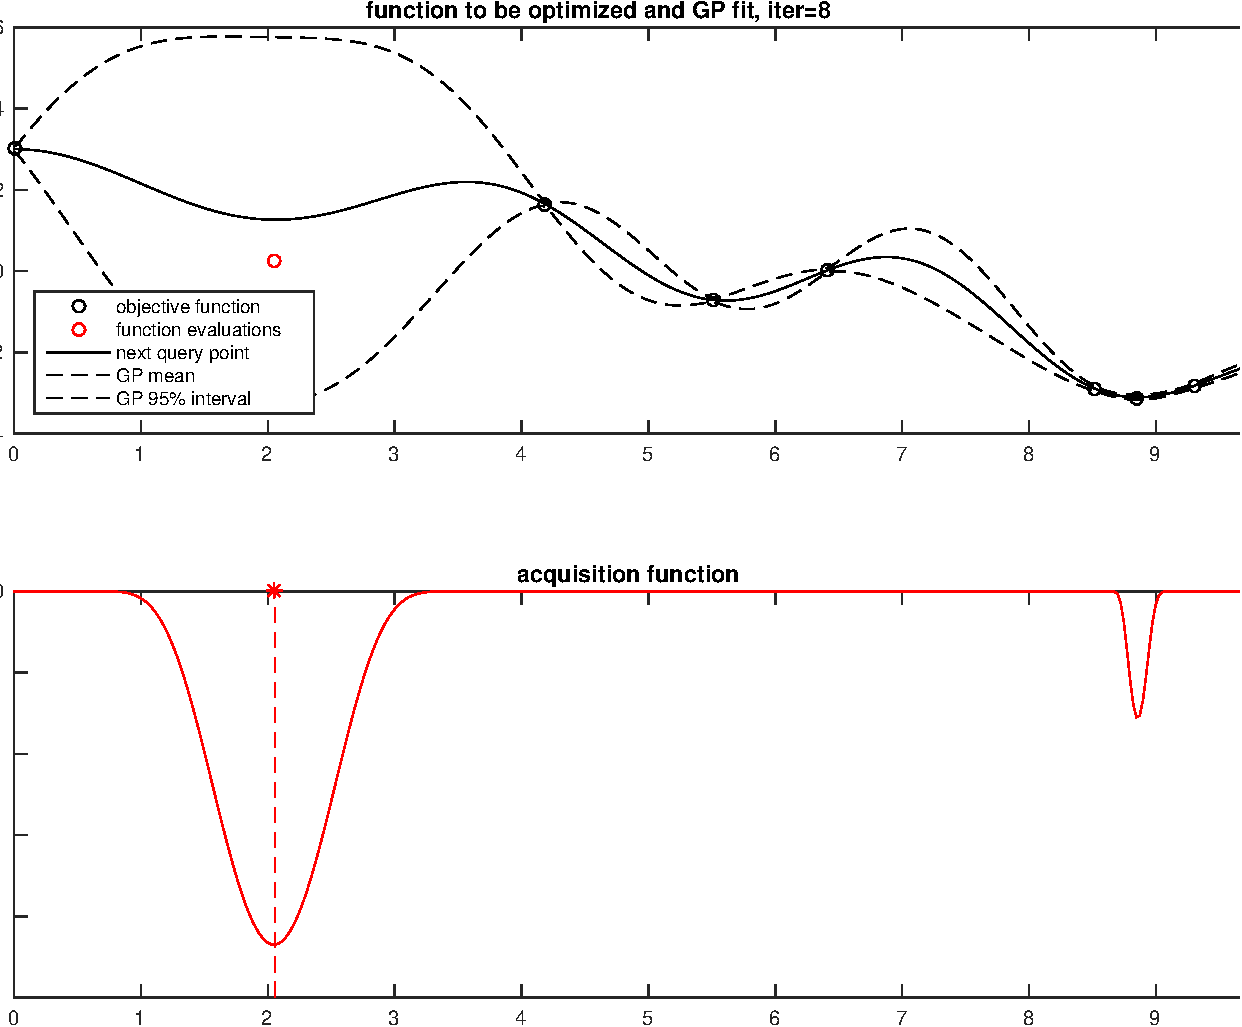
\includegraphics[width=10cm]{bayesopt_1d_regular_iter8-crop.pdf}

\end{frame}
\begin{frame}
  
  {\Large\color{navyblue} Bayesian optimization}

    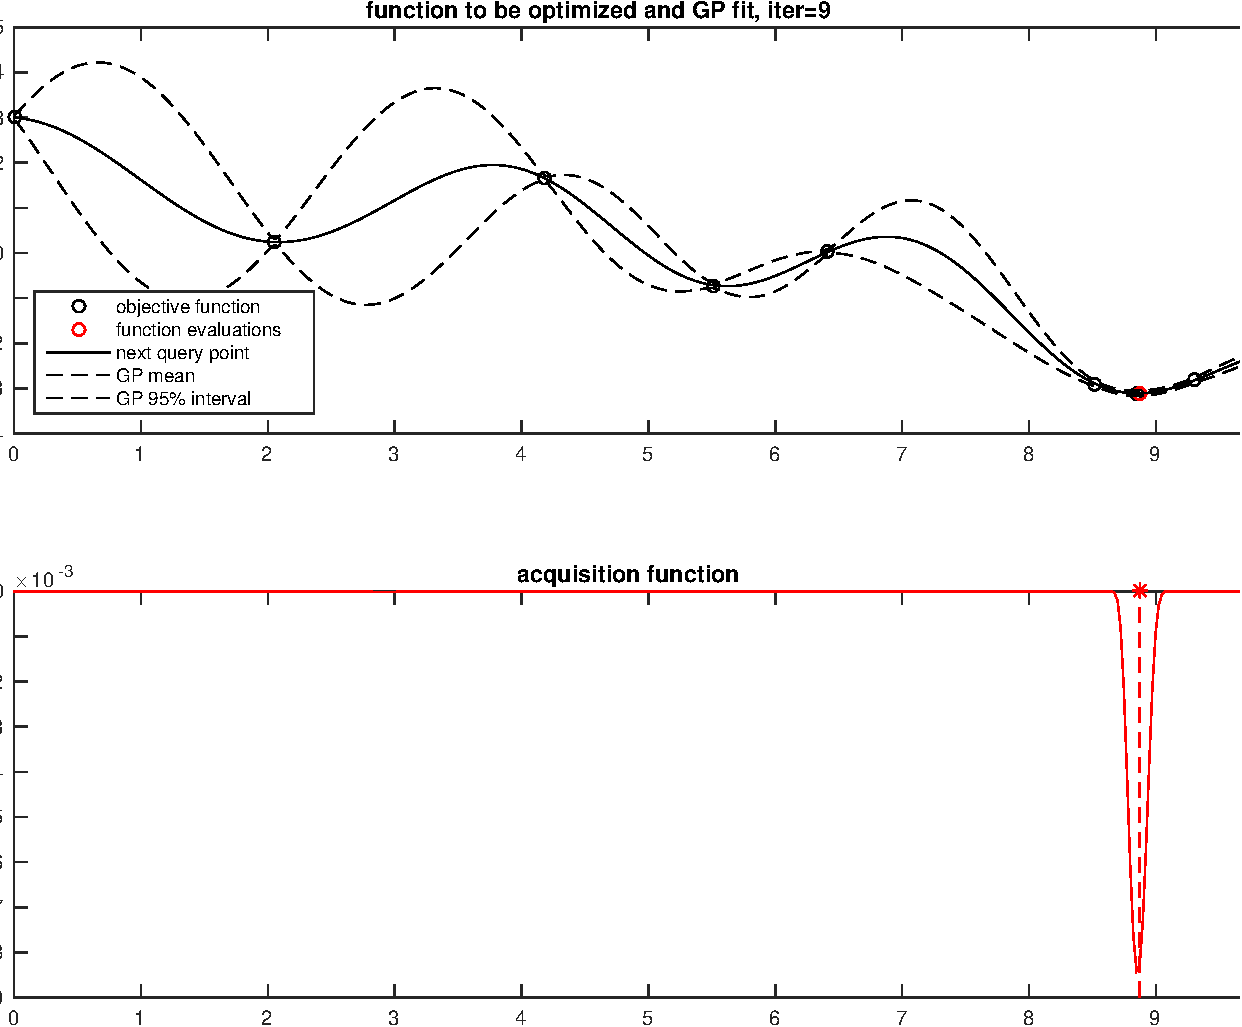
\includegraphics[width=10cm]{bayesopt_1d_regular_iter9-crop.pdf}

\end{frame}
\begin{frame}
  
  {\Large\color{navyblue} Bayesian optimization}

    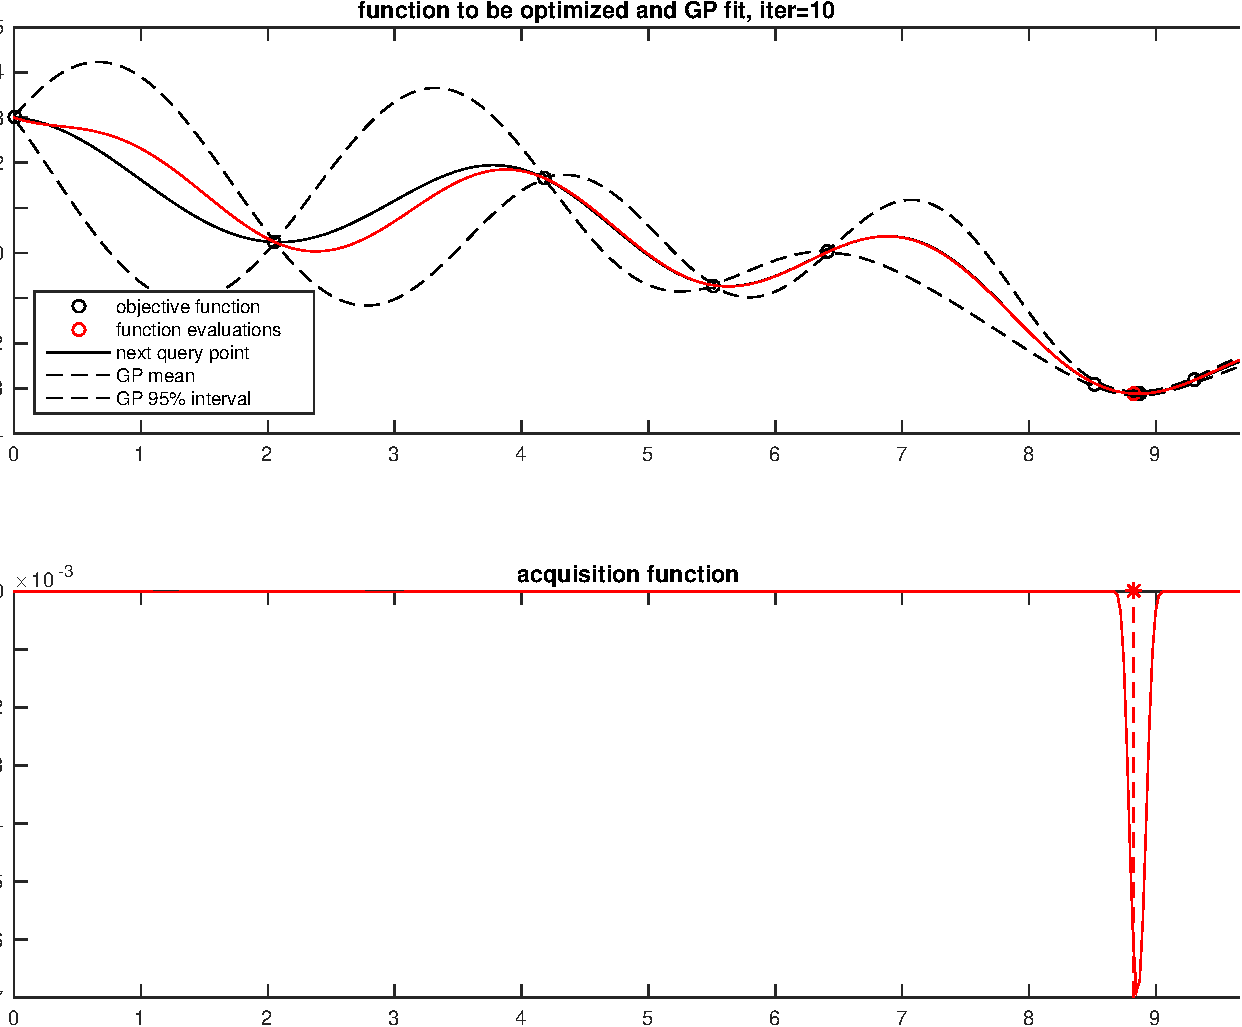
\includegraphics[width=10cm]{bayesopt_1d_regular_iter10-crop.pdf}

\end{frame}

\begin{frame}
  
  {\Large\color{navyblue} Model selection as decision problem}

  \begin{itemize}
  \item Expected utility of using the model in the future
  \end{itemize}

\end{frame}

\end{document}

%%% Local Variables:
%%% mode: latex
%%% TeX-master: t
%%% End:
